\documentclass[11pt]{article}
\usepackage[margin=1in]{geometry}
\usepackage[utf8]{inputenc}
\usepackage[T1]{fontenc}
\usepackage{times}
\usepackage{microtype}
\usepackage{amsmath,amssymb,amsthm}
\usepackage{booktabs}
\usepackage{graphicx}
\usepackage{xcolor}
\usepackage[numbers,sort&compress]{natbib}
\usepackage[colorlinks=true,linkcolor=blue!60!black,citecolor=blue!60!black,urlcolor=blue!60!black]{hyperref}
\usepackage[capitalize,noabbrev]{cleveref}

\newtheorem{proposition}{Proposition}
\title{\textbf{When Should a Process Label Expire?}}
\author{Manoj Bajaj}
\date{}
\hypersetup{pdftitle={When Should a Process Label Expire?},pdfauthor={Manoj Bajaj}}

\begin{document}
\maketitle
\begin{abstract}
Process verifiers can score an intermediate step for both legal execution and progress toward a solution.
A solver upgrade can change progress without changing legality, suggesting that the two fields should expire independently.
We preregistered an equal-budget test on 32 streams of bounded arithmetic puzzles, where a solver gains a continuation move and stale progress labels can be checked against exact enumeration.
At 96 operations per upgraded board, retaining legality and selectively refreshing progress improved exact joint-label accuracy by 0.02 percentage points over whole-label refresh (97.5\% paired interval: 0.001 to 0.037), but lost 0.37 points to memoized progress recomputation (\(-0.492\) to \(-0.241\)).
Both comparisons miss the 2-point promotion bar; all methods retained exact labels on unchanged boards.
The result separates the semantic case for two fields from the computational case for a separate expiration guard: in this finite setting, memoization was more useful than the guard.
\end{abstract}

\section{Introduction}

The useful next step in a reasoning trace depends on what the solver can do after taking it. A legally executed arithmetic move can be a detour for a solver that lacks a shortcut, then become useful once the solver gains it. Process advantage verifiers make that distinction by measuring progress against a specified continuation policy~\citep{setlur2024rewarding}. Step validity answers a different question: whether the move followed the task rules at all. If a verifier keeps both labels for future use, a solver release can make one field stale while leaving the other correct.

This suggests attaching different expiration conditions to the two fields. Keep a checked validity label while the grammar is unchanged, and refresh the progress label only when the new release may change a continuation it depends on. The semantic distinction is straightforward. The computational claim is not: a release can touch many continuation neighborhoods without changing their answers, and a recomputation baseline can share work across labels. To justify a row-level guard, selective refresh must beat both invalidating the whole guarded row and simply recomputing the solver-dependent part from a shared cache.

We test this claim in a bounded arithmetic task where legality is fixed, progress is exact, and the only change is a new continuation move. The guard has no false negatives for a release of this form. We compare three refresh policies at fixed operation caps against both a stale store and an independent oracle. A second release reverses the direction of the new move and increases how many labels change, without altering the task grammar.

The guard recovers stale labels, but its benefit does not clear the preregistered bar. On release A at the primary cap, split labels reach 96.53\% versus 96.51\% for whole-label refresh and 96.89\% for memoized recomputation (\cref{tab:primary}). The latter spends its budget on continuation attempts rather than screening rows. At a larger cap all three refresh policies reach exact labels on release A, while memoized recomputation spends fewer operations (\cref{fig:cap,sec:diagnostic}). This is a failure of the tested refresh primitive, not a reason to confuse validity with progress.

\begin{figure}[t]
\centering
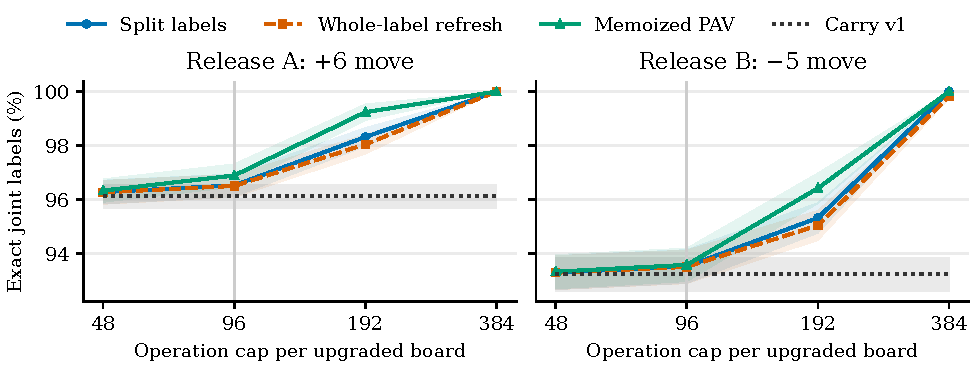
\includegraphics[width=\linewidth]{accuracy.pdf}
\caption{\textbf{Memoized recomputation is at least as accurate as guarded split refresh at every tested cap.}
Exact joint-label accuracy on upgraded arithmetic boards, averaged over 32 paired streams; bands show marginal 95\% stream-level intervals, not intervals for contrasts. The dotted horizontal line leaves labels at v1; the vertical marker indicates the primary cap, 96 operations per upgraded board. The right panel is the descriptive second release.}
\label{fig:cap}
\end{figure}

\section{A verifier with two label lifetimes}

Each board has states $x\in\{0,\ldots,23\}$ and one goal $g$.
For a candidate increment $d$, a legality verifier checks whether $y=x+d$
stays on the board. A separate continuation solver uses a set of increments
that may vary by state and release. Let $V_v^h(x)\in\{0,1\}$ indicate
whether solver release $v$ can reach $g$ from $x$ in at most $h$ moves.
A legal row $(x,d)$ has progress
\begin{equation}
  P_v(x,d) = V_v^4(x+d)-V_v^5(x).
  \label{eq:progress}
\end{equation}
An invalid row has no progress label. This is an exact reachability
analogue of a process advantage: the continuation prover searches
all eligible routes within its horizon rather than sampling completions
from a stochastic policy. Because the candidate legal moves are available
to the continuation solver, $P_v=0$ for a move that preserves reachability
(including a tie between two unsolvable states) and $P_v=-1$ for a move
that loses a reachable goal. The test measures whether those labels
remain correct, not whether every zero means a useful step.

\paragraph{Guard.}
Release v1 uses $+1,+3,-2$ at every state. The new positive or negative
shortcut in v2 is available only at states with residue $r$ modulo three
and only when its destination is legal. At v1, before the release,
the guard records which of the three residues can be reached by an old
trajectory with time left. It stores the union of these masks for the
two terms in \cref{eq:progress}, omitting a term if its old value is
already true. At release, check the bit for $r$ and refresh the label
only if that bit is set.

\begin{proposition}
If a row is not flagged, its joint label is exact under v2.
\end{proposition}
\begin{proof}
Legality does not depend on the solver. Adding a move leaves every old
successful path available. For an old-false term to become true, a new
successful path must use the added move at least once. Its prefix
before the first such move uses only old moves and reaches residue $r$
with at least one move left. The corresponding term must have
contributed the bit for $r$ to the stored mask.
\end{proof}

The converse is false. The new move can go off the board or fail to lead
to the goal, and simultaneous changes in the two reachability terms can
cancel. The guard uses the same old cache and release metadata as the controls:
whole-label refresh receives the same masks and serves the same v1
labels while work is pending. Its only extra charged work is rerunning
validity on a flagged row. The second control, memoized process advantage
verifier (PAV) recomputation,
preserves the independently cached validity and runs the same continuation
query code on every legal row without looking up a mask. All three refresh
arms share solver subproblems within a board and can skip old-true cells.
For comparison, carry leaves the two v1 fields in place, regardless of
release. \Cref{tab:axes} lists their differing work.

\begin{table}[h]
\centering
\caption{\textbf{The split and whole policies differ only on flagged legality work.}
Costs are per upgraded board before budget truncation. There are 66 legal
rows, of which $f$ are flagged. $S$ is the number of attempted
continuation moves, which can vary with the refresh policy. All arms
share the v1 cache.}
\label{tab:axes}
\begin{tabular}{lrrrr}
\toprule
Policy & Mask bytes & Guards & Legal checks & Continuations \\
\midrule
Carry v1 & 0 & 0 & 0 & 0 \\
Whole-label refresh & 96 & 66 & $f$ & $S$ \\
Split labels & 96 & 66 & 0 & $S$ \\
Memoized PAV & 0 & 0 & 0 & $S$ \\
\bottomrule
\end{tabular}
\end{table}

\section{Experiments}
\label{sec:results}

Each of 32 seeded streams contains 16 independent boards. Twelve receive
the upgrade and four keep their old solver. Each board has a uniform random
goal and residue, and a random row order fixed across policies. We label
every state crossed with $+1,+3,-2,+25$, including the goal state.
The always-illegal $+25$ gives an explicit invalid family in addition to
out-of-bounds cases of the other moves. The primary release adds $+6$;
the secondary release instead adds $-5$ to the same paired boards.
Each cap is applied independently per upgraded board. A guard lookup,
rerun of a legality check, or attempted continuation move costs one
operation; no method can charge a partially finished row as refreshed.
The outcome is exact joint labels, not reward accuracy on solver outputs.

\paragraph{Positive control.}
The independent labeler expands reached-state sets forward, rather than
memoizing backward reachability. All three refresh arms match it on all
1,536 arm--board checks for each release when the cap is removed, including
unreleased boards. Freezing the store leaves 1,429 of 36,864 upgraded rows
wrong after release A (3.88\%) and 2,497 wrong after release B (6.77\%).
The primary release therefore exceeds the required 1-point stale-label
error before testing any proposed improvement.

\begin{table}[h]
\centering
\caption{\textbf{Bypassing the guard uses more of the cap for continuation work.}
Release A, primary cap of 96 operations per upgraded board. Exact joint
accuracy is a mean with 95\% marginal $t$ intervals over 32 streams; work
columns are means per upgraded board. Paired contrasts are given in text.}
\label{tab:primary}
\begin{tabular}{lrrrrr}
\toprule
Policy & Exact (\%) $\uparrow$ & Total & Guard & Validity & Continuation \\
\midrule
\csname @@input\endcsname table_accuracy.tex
\bottomrule
\end{tabular}
\end{table}

\paragraph{Primary test.}
At 96 operations per upgraded board, guarded split refresh gains
0.019 percentage points over whole-label refresh (97.5\% paired
interval: 0.001 to 0.037), but loses 0.366 points to memoized PAV
(\(-0.492\) to \(-0.241\)). These are the preregistered two-sided
intervals, giving 95\% familywise coverage by Bonferroni. Both upper
bounds fall below the required 2-point gain. This is not an inability to
resolve a noisy tie: the interval against memoized PAV lies entirely below
zero, and even the upper bound against whole-label refresh is close to zero
relative to the decision threshold.

\paragraph{Retention.}
At the primary cap, all four policies retained all 12,288 unchanged rows,
all 15,360 invalid rows across both upgraded and unchanged boards, and all
3,072 unchanged statewise weak orderings, including ties.
All 986 strict detours (unchanged rows with $P_1=-1$) retained their old
label exactly. These are intended invariances: the release does not touch task
legality or the solver on those boards. They check for collateral damage to
the label store, not generalization of a learned verifier.

\subsection{Where did the budget go?}
\label{sec:diagnostic}

Both guards mark 9,298 rows as potentially stale, 36.7\% of the legal
rows on upgraded boards. They cover all actual changes, but only 15.4\%
of flags correspond to changed labels in release A and 26.9\% in B.
The guard detects access to a new move rather than a change in reachability,
and progress can stay the same even when a reachability term changes.
Guard charges at the primary cap cost split refresh 8.76 operations per
board on average, while whole-label refresh spent just 2.24 on legality.
The gain from skipping that check is small in an arithmetic grammar; the
unguarded baseline spends almost all available work on shared continuation
queries instead (\cref{tab:primary}).

At the 384-operation cap in release A, guarded split refresh and memoized
recomputation both recover every joint label and spend the same 180.18
mean continuation attempts. The guarded version spends 66 more operations
per board, exactly one lookup per legal row. This does not imply pruning
can never save search. In this store, unflagged rows did not add to the
aggregate continuation work once queries were shared, so pruning those
rows did not save enough work to amortize the guard.

\paragraph{Second release.}
The negative move creates more stale labels but does not reverse the
comparison at the primary cap: split leads whole-label refresh by 0.016
points and trails memoized recomputation by 0.060 points. At the largest
cap split and memoized recomputation reach exact labels while whole
remains at 99.82\%. These comparisons are descriptive, not a second
promotion test. \Cref{fig:cap} shows the complete budget sweep.

\section{Related work}

\paragraph{What a step label means.}
Process supervision uses judgments of intermediate steps rather than
only grading final answers~\citep{lightman2023verify}. Rewarding Progress
defines progress by a separate prover's change in success
probability~\citep{setlur2024rewarding}. Our bounded reachability
label is a deterministic analogue; we ask how to maintain that label
when the prover changes, not whether training on progress improves
reasoning. Keeping validity and progress separate is compatible with
that baseline and is not by itself evidence for a guard.

\paragraph{Maintaining answers after a release.}
Incremental path algorithms address what to recompute after a graph
update~\citep{ramalingam1996incremental}. Our mask is more limited: it
certifies that a row cannot change under an additive release with a
specified source class, without maintaining paths or reverse dependencies.
The memoized PAV baseline is intentionally simpler than a fully
incremental graph algorithm. The test asks whether the row certificate
adds value even against this relatively cheap alternative.

\section{Conclusion}

Separating legality from progress describes the arithmetic verifier
correctly, but it does not establish a useful expiration primitive.
The guard catches every changed label, yet spends budget on many rows
whose labels stay correct. Exact progress recomputation from a shared
cache makes better use of the same budget on the primary release;
whole-label refresh is only marginally behind the split variant.
We do not promote split expiry on this evidence.

The experiment assumes known additive solver edits, fixed step legality
and perfect legality checks that are cheap to repeat; the retention
slice deliberately does not change. The test bounds usefulness in this
finite setting, not in language-model systems whose checks may rely on
expensive tools or whose continuation policies cannot be enumerated.
For a guard to be worth testing there, it should have measurable
precision, and the search it saves must exceed guard cost after
cross-row memoization. Changes that remove continuations or change
the grammar would also require a different soundness argument.

The preregistration, runner, tests and per-stream results are in the
repository's experiment directory; the plot and table can be regenerated
from the saved results without rerunning the pilot.


\section*{AI use}
Idea selection was mixed: Manoj Bajaj directed the research program and its idea pool; Devin (Cognition AI) selected and operationalized the card for this study.
Devin conducted the literature check, designed and ran the experiments, analyzed the results, and wrote and typeset the paper, without a separate human review of the PDF.

\bibliographystyle{plainnat}
\setlength{\bibsep}{2pt}
\bibliography{references}
\clearpage
\appendix
\section{Reproduction details}
\label{app:details}

The test uses CPU-only Python 3.10.12, NumPy 2.2.6 with PCG64 seeds 0--31,
and SciPy 1.15.3. There are no trainable parameters or fitting steps.
The saved run took about seven seconds on an Intel Xeon VM across both
releases, all caps and arms, and the independent oracle checks.
From the repository root, run:
\begin{verbatim}
cd experiments/split-lifetime-labels
python -m unittest -v
python run.py
cd ../../papers/split-lifetime-labels
python plot.py
latexmk -pdf -interaction=nonstopmode -halt-on-error paper.tex
\end{verbatim}
The protocol was committed before the first run
(\href{https://github.com/manojbajaj95/cl/commit/e95e61a}{\texttt{e95e61a}}).
The runner writes one record for each seed per release, preserves all
retention and work counts, and reports the decision computed from the
two prespecified paired contrasts. Stream-level estimates first average
over boards within each stream. Since their board and row counts are
equal, this gives the same point estimate as pooling rows but uses
streams, not pooled rows, as replicates for the intervals.

\paragraph{Cached state and cost scope.}
All arms may retain the 96 baseline rows, each containing validity and
an optional signed progress bit of information, and the $6\times24$
Boolean v1 reachability table. The Python code represents them as
lists and tuples; Python object sizes are not treated as transmission
costs. The guard is a 96-byte payload per board. The temporary v2
memo is keyed by the remaining horizon and integer state, with at most
$5\times24$ entries. Old-cache construction, fixed indexing, and
in-memory row writes are excluded from the work-unit budget and both
check and continuation attempts are charged the same. These choices
favor the guarded policies insofar as they also need extra v1 mask
compilation. No wall-clock superiority is
inferred from the operation comparisons.

\paragraph{Two ways to compute reachability.}
The recomputation queries $V_v^h(x)$ recursively, using the previous
value immediately when $h=0$ or the cell was true at v1. Otherwise it
tries old moves in the order $+1,+3,-2$, then the new move where
eligible, memoizing each completed cell. The oracle instead starts
with $\{x\}$, unions in every state reachable by one move at each
iteration, and checks goal membership after $h$ iterations; it uses
neither v1 reuse nor the guard. Budget exhaustion leaves the current
row unchanged and stops the upgrade work for the board.

\end{document}
